\documentclass[a4paper,11pt]{article}
\usepackage[utf8]{inputenc}
\usepackage[T1]{fontenc}
\usepackage[czech]{babel}
\usepackage{lmodern}
\usepackage{booktabs}
\usepackage{array}
\usepackage{xcolor}
\usepackage{graphicx}
\usepackage{tikz}
\usetikzlibrary{positioning,arrows.meta}
\usepackage[hidelinks]{hyperref}
\setlength{\emergencystretch}{3em}
\usepackage[left=2cm,right=2cm,top=2.5cm,bottom=2.5cm]{geometry}
\usepackage{longtable}
\usepackage{pdflscape}
\usepackage{float}

\newcommand{\nt}[1]{$\langle$\textit{#1}$\rangle$}   % neterminál
\newcommand{\tk}[1]{\texttt{#1}}                     % terminál (token lexeru)
\newcommand{\pt}[1]{\texttt{\textbf{#1}}}            % pseudo-terminál (výraz)
\newcommand{\grp}[1]{\textsf{\textbf{#1}}}           % skupina tokenů (legenda)
\newcommand{\rot}[1]{\rotatebox{90}{#1}}
\providecommand{\code}[1]{\texttt{#1}}
 
\begin{document}
 
%======================================================================
% Titulní strana
%======================================================================
\begin{titlepage}
  \centering
  {\Large Vysoké učení technické v~Brně\\Fakulta informačních technologií\par}
  \vspace{4cm}
  {\LARGE Dokumentace projektu do předmětů IFJ a IAL\par}
  \vspace{0.5cm}
  {\Huge\bfseries Implementace překladače jazyka IFJ26\par}
  \vspace{1.5cm}
  {\Large Tým: xkralil00\par}
  \vspace{0.3cm}
  {\Large Varianta: TRP-izp\par}
  \vspace{2cm}
 
  \begin{tabular}{l l l r}
    \toprule
    Jméno a příjmení & Login & Osobní číslo & Body \\
    \midrule
    {\textbf{Lukáš Králíček}} & \texttt{\textbf{xkralil00}} & \textbf{282310} & 25 \% \\
    {Anežka Alexis Kohelová} & \texttt{xkohela00} & 282487 & 25 \% \\
    {David Bosák} & \texttt{xbosakd00} & 282175 & 25 \% \\
    {Jakub Mejstřík} & \texttt{xmejstj00} & 281972 & 25 \% \\
    \bottomrule
  \end{tabular}
 
  \vspace{1.5cm}
  \begin{center}
    Implementovaná rozšíření: \texttt{BOOLTHEN, CONTROL, FUNEXP} \\
    Git repozitář: https://github.com/SusenkaOREOcze/nejlepsiprekladacever-ifj-proj-2026 \\
  \end{center}
 
  \vfill
  {{27.11.2026}\par}
\end{titlepage}
 
\tableofcontents
\newpage
 
%======================================================================
\section{Rozdělení práce}
%======================================================================
 
\begin{itemize}
  \item \texttt{xkralil00} -- \textbf{Vedoucí projektu},  lexikální analyzátor, tvorba AST a TAC, tvorba irgen
  \item \texttt{xbosakd00} -- tabulka s rozptýlenými položkami, tabulka symbolů a tabulka funkcí, generátor výsledného kódu
  \item \texttt{xmejstj00} -- sémantická analýza, LL gramatika, dokumentace
  \item \texttt{xkohela00} -- syntaktická analýza, stavba AST, precedenční tabulka
\end{itemize}

 
%======================================================================
\section{Spolupráce, testování a styl kódu}
%======================================================================
 
\paragraph{Spolupráce a code review.}
Tým pracoval na vlastních větvích projektu. Všechny PR do main větve musely být schváleny všemi členy. Další dodatečné úpravy nebo opožděná komunikace byly komunikovány přes týmový Discord.
 
\paragraph{Testování.}
    Pro celý projekt byl použit testovací framework Cmocka~\cite{cmoccka}. Pro spuštění testů je použit příkaz \texttt{make test}. Paměť je testována za pomoci AddressSanitizer.
 
\paragraph{Styl kódu.} Pro formátování a správu názvů bylo použito \texttt{clang-format} a \texttt{clang-tidy}.
\begin{itemize}
    \item Pravidla formátování kódu: LLVM
    \item Styl odsazení: Tabulátor
    \item Délka odsazení: 4
    \item Počet znaků na řádku: 110
\end{itemize}

%======================================================================
\section{Architektura překladače}
%======================================================================

Lexikální analyzátor čte zdrojový program ze standardního vstupu a na požádání parseru vrací tokeny (struktura \texttt{token\_t}). Parser provádí pouze syntaktickou analýzu a hlásí události AST builderu, který poté staví AST zdola nahoru. Sémantická analýza poté prochází AST a zapisuje typy a \verb|symbol_id|, při tom využívá tabulku symbolů a funkcí. Obě tabulky stojí nad TRP. Z doplněného AST vytvoří generátor mezikódu tříadresný kód TAC a převede se na IFJcode26 a je to výstup na stdout. Každá fáze končí při první chybě. Překladač neobsahuje optimalizátor kódu.
 
\begin{figure}[H]
  \centering
  \begin{tikzpicture}[
    node distance=1.4cm and 2.6cm,
    mod/.style={draw, rounded corners, minimum width=3.6cm, minimum height=1cm, align=center},
    dat/.style={draw, dashed, minimum width=3.6cm, minimum height=0.9cm, align=center},
    io/.style={align=center},
    arr/.style={-{Latex}, thick},
    lbl/.style={font=\small, align=center}
    ]
        \node[io](in) {zdrojový program\\(\texttt{stdin})};
        \node[mod, below=of in](lex){lexikální analýza};
        \node[mod, below=of lex](par){syntaktická analýza\\(LL + precedenční)};
        \node[mod, below=of par](ast){AST builder};
        \node[mod, right=of ast](sem){sémantická analýza};
        \node[dat, above=of sem](tab){tabulka symbolů (\texttt{symtable})\\
            tabulka funkcí (\texttt{functable})\\[2pt] {\footnotesize tabulka s rozptýlenými položkami}};
        \node[mod, below=of sem](ir){generátor mezikódu\\(irgen)};
        \node[mod, below=of ir](gen){generátor cílového kódu};
        \node[io,  below=of gen](out){program v~IFJcode26\\(\texttt{stdout})};

        \draw[arr] (in)  -- (lex);
        \draw[arr] (lex) -- node[lbl, left] {tokeny (\texttt{token\_t}):\\aktuální + následující} (par);
        \draw[arr] (par) -- node[lbl, left] {události\\\texttt{syntax\_semantic\_action}\\(v postfixovém pořadí)} (ast);
        \draw[arr] (ast) -- node[lbl, above] {AST (\texttt{ast\_t})} (sem);
        \draw[arr, <->] (sem) -- node[lbl, left] {\texttt{symt\_t},\\\texttt{funct\_t}} (tab);
        \draw[arr] (sem) -- node[lbl, left] {anotovaný AST\\(typy, \texttt{symbol\_id})} (ir);
        \draw[arr] (ir) -- node[lbl, left] {mezikód (TAC)} (gen);
        \draw[arr] (gen) -- (out);
    \end{tikzpicture}
    \caption{Blokové schéma překladače}
    \label{fig:architektura}
\end{figure}
 
%====================================================================== 
\section{Konečný automat lexikálního analyzátoru}
%======================================================================
Lexer je implementován jako rozšířený deterministický konečný automat (obrázek~\ref{fig:automat}). Každé volání \texttt{lexer\_scan\_token} začíná ve stavu \textsc{scan}, podle prvního znaku se rozhodne pro třídu tokenu a uvnitř ní čte nejdelší možný lexém.
\\
\\
\textbf{Odchylky od standardního modelu konečného automatu:}
\begin{itemize}
    \item přechod může mít v~hranatých závorkách podmínku, např.\ hloubku odsazení,
    \item automat může nahlédnout na další znak, aniž by jej spotřeboval. Náhled se provede funkcí \texttt{fgetc} a znak se vrátí funkcí \texttt{ungetc}. Náhled o jeden znak je možný z definice~\cite{ungetc},
    \item mezi voláními si automat pamatuje čítače: zásobník šířek odsazení, hloubku závorek, hloubku vnoření komentářů a počet dosud nevydaných tokenů \texttt{DEDENT},
    \item identifikátory a čísla jsou na hranách zapsány regulárním výrazem, který zastupuje posloupnost stavů a přechodů,
    \item \textsc{token} a \textsc{error} jsou koncové stavy jednoho volání. Další volání začíná opět ve stavu \textsc{scan} a čítače si ponechává,
\end{itemize}
Pro zjednodušení DKA byla navržena verze pokrývající všechny stavy a přechody. Ovšem pro čitelnost byly všechny přechody očíslovány. Korespondující názvy jsou poté obsaženy v \textbf{~Tabulce~1:~Přechody~konečného~automatu~lexikálního~analyzátoru.}
\newpage
\begin{landscape}
\begin{figure}[h]
    \centering
    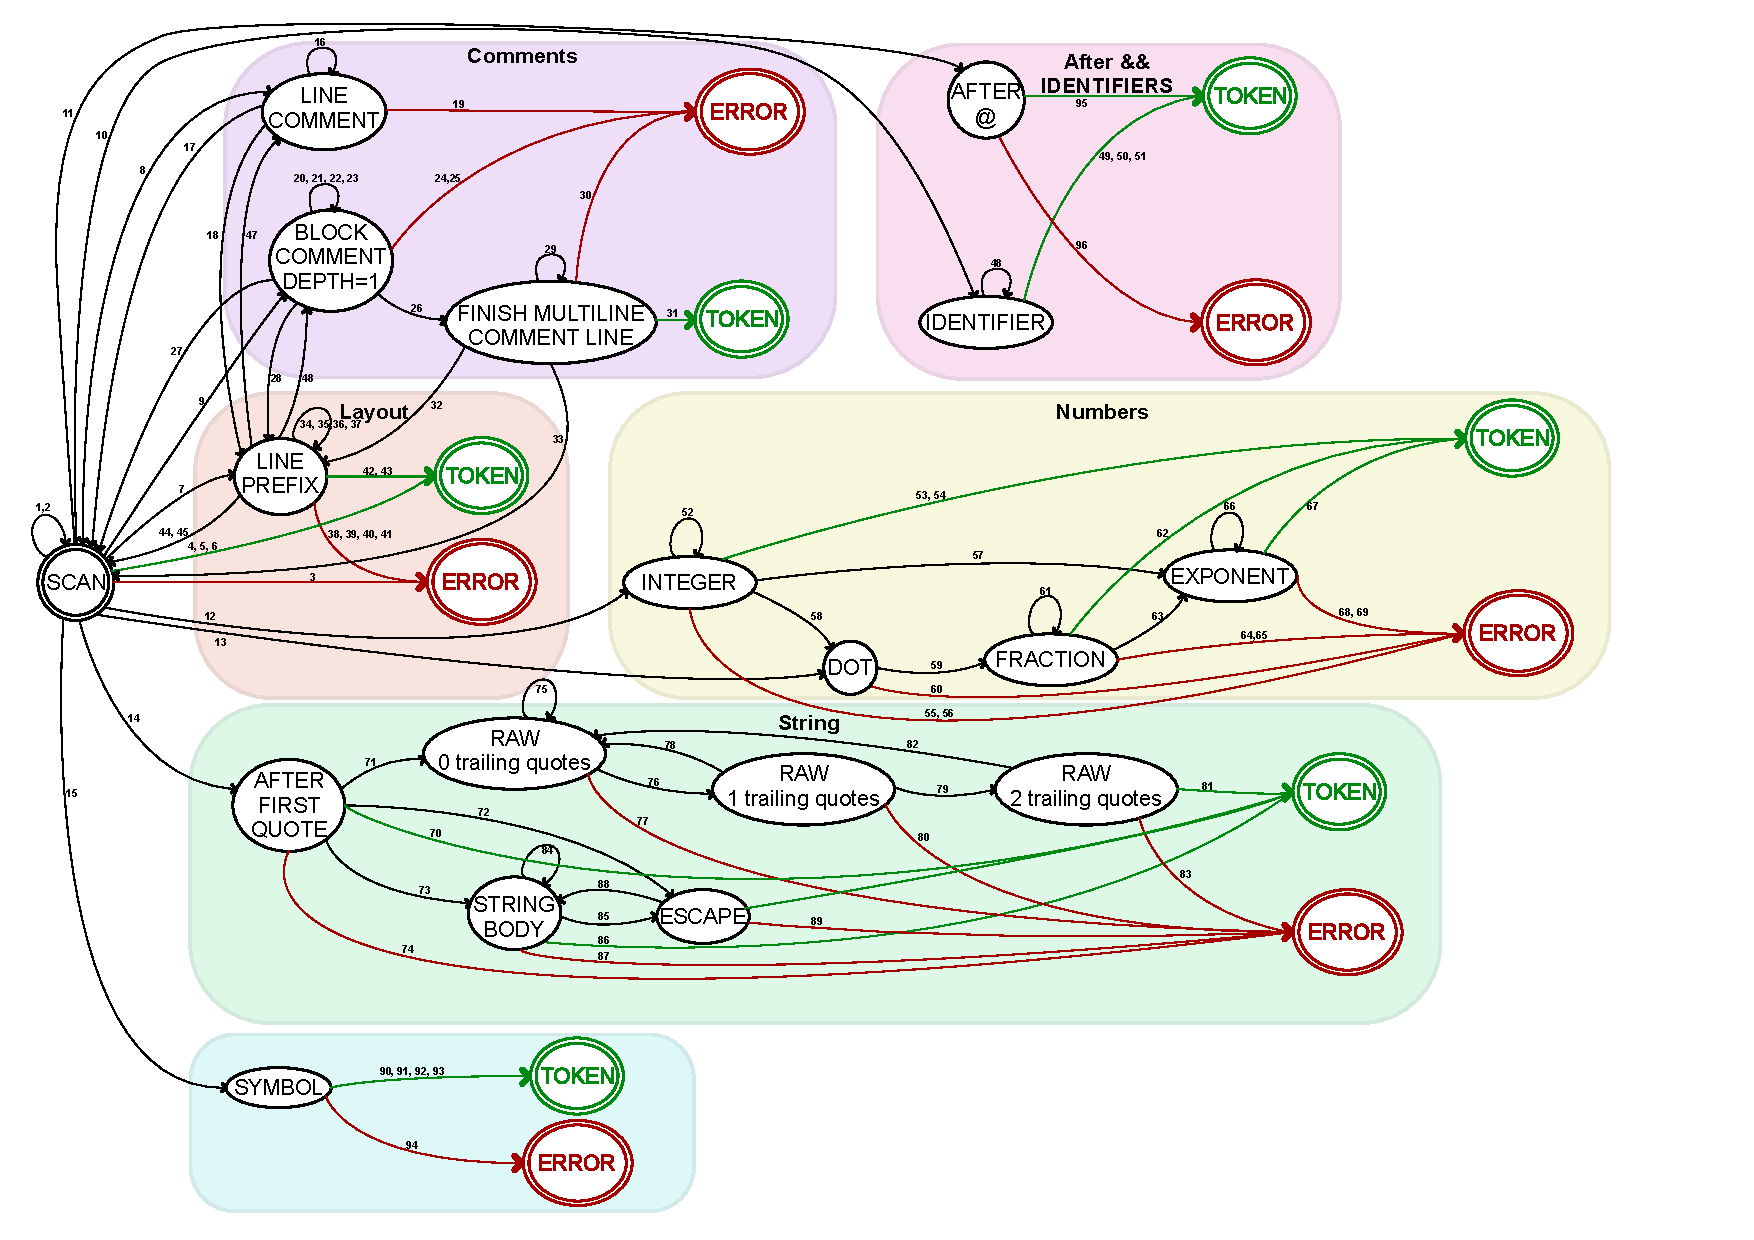
\includegraphics[width=25.5cm]{lexerDKA.pdf}
    \caption{Konečný automat lexikálního analyzátoru}
  \label{fig:automat}
\end{figure}
\end{landscape}
\begin{landscape}
{\small
\setlength{\tabcolsep}{3pt}
\begin{longtable}{@{}r >{\raggedright\arraybackslash}p{4.0cm} >{\raggedright\arraybackslash}p{9.8cm} >{\raggedright\arraybackslash}p{5.4cm}>{\raggedright\arraybackslash}p{4.0cm}@{}}
\caption{Přechody konečného automatu lexikálního analyzátoru}
\label{tab:prechody}\\
\toprule
\textbf{č.} & \textbf{Ze stavu} & \textbf{Vstup [podmínka]} & \textbf{Akce / výstup} & \textbf{Do stavu} \\
\midrule
\endfirsthead
\toprule
\textbf{č.} & \textbf{Ze stavu} & \textbf{Vstup [podmínka]} & \textbf{Akce / výstup} & \textbf{Do stavu} \\
\midrule
\endhead
\bottomrule
\endfoot
\multicolumn{5}{@{}l}{\textbf{Start -- SCAN}} \\*
1 & SCAN & \texttt{{[}\ \textbackslash{}t{]}\allowbreak{}} & -- & SCAN \\
2 & SCAN & \texttt{\textbackslash{}n} \texttt{{[}lexer-{}\textgreater{}parenthesis\_depth\textgreater{}0{]}\allowbreak{}} & \texttt{lexer-{}\textgreater{}at\_line\_start=true} & SCAN \\
3 & SCAN & \texttt{{[}\textasciicircum{}ASCII{]}\allowbreak{}\textbar{}\allowbreak{}\textbackslash{}r} & \texttt{ERROR} & ERROR \\
4 & SCAN & \texttt{EOF} \texttt{{[}indent\_count\textgreater{}0{]}\allowbreak{}} & \texttt{TOKEN\_DEDENT} & TOKEN \\
5 & SCAN & \texttt{\textbackslash{}n} \texttt{{[}lexer-{}\textgreater{}parenthesis\_depth==0{]}\allowbreak{}} & \texttt{lexer-{}\textgreater{}at\_line\_start=true,\allowbreak{}\ TOKEN\_NEWLINE} & TOKEN \\
6 & SCAN & \texttt{EOF} \texttt{{[}indent\_count==0{]}\allowbreak{}} & \texttt{TOKEN\_EOF} & TOKEN \\
7 & SCAN & \texttt{(?={[}ASCII{]}\allowbreak{})\allowbreak{}\textbar{}\allowbreak{}EOF} \texttt{{[}at\_line\_start{]}\allowbreak{}} & -- & LINE PREFIX \\
8 & SCAN & \texttt{{[}/{]}\allowbreak{}\{2\}} & -- & LINE COMMENT \\
9 & SCAN & \texttt{{[}/{]}\allowbreak{}{[}*{]}\allowbreak{}} & \texttt{*contains\_newline=false,\allowbreak{}\ lexer-{}\textgreater{}comment\_depth=1} & BLOCK COMMENT \\
10 & SCAN & \texttt{{[}A-{}Za-{}z\_{]}\allowbreak{}} & -- & IDENTIFIER \\
11 & SCAN & \texttt{@} & -- & AFTER @ \\
12 & SCAN & \texttt{{[}0-{}9{]}\allowbreak{}} & -- & INTEGER \\
13 & SCAN & \texttt{\textbackslash{}.(?={[}0-{}9{]}\allowbreak{})\allowbreak{}} & -- & DOT \\
14 & SCAN & \texttt{\textquotedbl{}} & -- & AFTER FIRST QUOTE \\
15 & SCAN & \texttt{(?!{[}A-{}Za-{}z\_0-{}9\textquotedbl{}@\ \textbackslash{}t\textbackslash{}r\textbackslash{}n{]}\allowbreak{}\textbar{}\allowbreak{}\textbackslash{}.(?={[}0-{}9{]}\allowbreak{})\allowbreak{}\textbar{}\allowbreak{}{[}/{]}\allowbreak{}{[}/*{]}\allowbreak{})\allowbreak{}{[}ASCII{]}\allowbreak{}} & -- & SYMBOL \\ 
\midrule
\multicolumn{5}{@{}l}{\textbf{Comments}} \\*
16 & LINE COMMENT & \texttt{(?!\textbackslash{}n)\allowbreak{}{[}ASCII{]}\allowbreak{}} & -- & LINE COMMENT \\
17 & LINE COMMENT & \texttt{(?=\textbackslash{}n)\allowbreak{}\textbar{}\allowbreak{}EOF} \texttt{{[}!at\_line\_start{]}\allowbreak{}} & -- & SCAN \\
18 & LINE COMMENT & \texttt{(?=\textbackslash{}n)\allowbreak{}\textbar{}\allowbreak{}EOF} \texttt{{[}at\_line\_start{]}\allowbreak{}} & \texttt{*width=0,\allowbreak{}\ has\_tab=false,\allowbreak{}\ count\_indentation=true} & LINE PREFIX \\
19 & LINE COMMENT & \texttt{{[}\textasciicircum{}ASCII{]}\allowbreak{}} & \texttt{ERROR} & ERROR \\
20 & BLOCK COMMENT & \texttt{(?!(?:{[}/{]}\allowbreak{}{[}*{]}\allowbreak{}\textbar{}\allowbreak{}{[}*{]}\allowbreak{}{[}/{]}\allowbreak{}\textbar{}\allowbreak{}\textbackslash{}n)\allowbreak{})\allowbreak{}{[}ASCII{]}\allowbreak{}} & -- & BLOCK COMMENT \\
21 & BLOCK COMMENT & \texttt{\textbackslash{}n} & \texttt{*contains\_newline=true} & BLOCK COMMENT \\
22 & BLOCK COMMENT & \texttt{{[}*{]}\allowbreak{}{[}/{]}\allowbreak{}} \texttt{{[}lexer-{}\textgreater{}comment\_depth\textgreater{}1{]}\allowbreak{}} & \texttt{-{}-{}lexer-{}\textgreater{}comment\_depth} & BLOCK COMMENT \\
23 & BLOCK COMMENT & \texttt{{[}/{]}\allowbreak{}{[}*{]}\allowbreak{}} \texttt{{[}lexer-{}\textgreater{}comment\_depth\textless{}SIZE\_MAX{]}\allowbreak{}} & \texttt{++lexer-{}\textgreater{}comment\_depth} & BLOCK COMMENT \\
24 & BLOCK COMMENT & \texttt{{[}/{]}\allowbreak{}{[}*{]}\allowbreak{}} \texttt{{[}lexer-{}\textgreater{}comment\_depth==SIZE\_MAX{]}\allowbreak{}} & \texttt{ERROR} & ERROR \\
25 & BLOCK COMMENT & \texttt{{[}\textasciicircum{}ASCII{]}\allowbreak{}\textbar{}\allowbreak{}EOF} & \texttt{ERROR} & ERROR \\
26 & BLOCK COMMENT & \texttt{{[}*{]}\allowbreak{}{[}/{]}\allowbreak{}} \texttt{{[}lexer-{}\textgreater{}comment\_depth==1,\allowbreak{}\ *contains\_newline{]}\allowbreak{}} & \texttt{-{}-{}lexer-{}\textgreater{}comment\_depth} & FINISH MULTILINE COMMENT LINE \\
27 & BLOCK COMMENT & \texttt{{[}*{]}\allowbreak{}{[}/{]}\allowbreak{}} \texttt{{[}comment\_depth==1,\allowbreak{}\ !contains\_newline,\allowbreak{}\ !at\_line\_start{]}\allowbreak{}} & \texttt{-{}-{}comment\_depth} & SCAN \\
28 & BLOCK COMMENT & \texttt{{[}*{]}\allowbreak{}{[}/{]}\allowbreak{}} \texttt{{[}comment\_depth==1,\allowbreak{}\ !contains\_newline,\allowbreak{}\ at\_line\_start{]}\allowbreak{}} & \texttt{-{}-{}comment\_depth,\allowbreak{}\ count\_indentation=false} & LINE PREFIX \\
29 & FINISH MULTILINE COMMENT LINE & \texttt{{[}\ \textbackslash{}t{]}\allowbreak{}} & -- & FINISH MULTILINE COMMENT LINE \\
30 & FINISH MULTILINE COMMENT LINE & \texttt{{[}\textasciicircum{}\ \textbackslash{}t\textbackslash{}n{]}\allowbreak{}} & \texttt{ERROR} & ERROR \\
31 & FINISH MULTILINE COMMENT LINE & \texttt{\textbackslash{}n\textbar{}\allowbreak{}EOF} \texttt{{[}!at\_line\_start,\allowbreak{}\ parenthesis\_depth==0{]}\allowbreak{}} & \texttt{TOKEN\_NEWLINE} & TOKEN \\
32 & FINISH MULTILINE COMMENT LINE & \texttt{\textbackslash{}n\textbar{}\allowbreak{}EOF} \texttt{{[}at\_line\_start{]}\allowbreak{}} & \texttt{*width=0,\allowbreak{}\ has\_tab=false,\allowbreak{}\ count\_indentation=true} & LINE PREFIX \\
33 & FINISH MULTILINE COMMENT LINE & \texttt{\textbackslash{}n\textbar{}\allowbreak{}EOF} \texttt{{[}!at\_line\_start,\allowbreak{}\ parenthesis\_depth\textgreater{}0{]}\allowbreak{}} & \texttt{at\_line\_start=true} & SCAN \\
\midrule
\multicolumn{5}{@{}l}{\textbf{Layout}} \\*
34 & LINE PREFIX & \texttt{\textbackslash{}n} & \texttt{*width=0,\allowbreak{}\ has\_tab=false,\allowbreak{}\ count\_indentation=true} & LINE PREFIX \\
35 & LINE PREFIX & \texttt{{[}\ \textbackslash{}t{]}\allowbreak{}} \texttt{{[}!count\_indentation{]}\allowbreak{}} & -- & LINE PREFIX \\
36 & LINE PREFIX & \texttt{\textbackslash{}t} \texttt{{[}count\_indentation{]}\allowbreak{}} & \texttt{has\_tab=true} & LINE PREFIX \\
37 & LINE PREFIX & \texttt{{[}\ {]}\allowbreak{}} \texttt{{[}count\_indentation{]}\allowbreak{}} & \texttt{++*width} & LINE PREFIX \\
38 & LINE PREFIX & \texttt{\textbackslash{}r} & \texttt{ERROR} & ERROR \\
39 & LINE PREFIX & \texttt{(?=(?!{[}/{]}\allowbreak{}{[}/*{]}\allowbreak{}\textbar{}\allowbreak{}{[}\ \textbackslash{}t\textbackslash{}r\textbackslash{}n{]}\allowbreak{})\allowbreak{}{[}ASCII{]}\allowbreak{})\allowbreak{}} \texttt{{[}has\_tab{]}\allowbreak{}} & \texttt{ERROR} & ERROR \\
40 & LINE PREFIX & \texttt{(?=(?!{[}/{]}\allowbreak{}{[}/*{]}\allowbreak{}\textbar{}\allowbreak{}{[}\ \textbackslash{}t\textbackslash{}r\textbackslash{}n{]}\allowbreak{})\allowbreak{}{[}ASCII{]}\allowbreak{})\allowbreak{}} \texttt{{[}parenthesis\_depth\textgreater{}0,\allowbreak{}\ width\textless{}=logical\_line\_indent{]}\allowbreak{}} & \texttt{ERROR} & ERROR \\
41 & LINE PREFIX & \texttt{(?=(?!{[}/{]}\allowbreak{}{[}/*{]}\allowbreak{}\textbar{}\allowbreak{}{[}\ \textbackslash{}t\textbackslash{}r\textbackslash{}n{]}\allowbreak{})\allowbreak{}{[}ASCII{]}\allowbreak{})\allowbreak{}} \texttt{{[}parenthesis\_depth==0,\allowbreak{}\ width\textless{}current\_width,\allowbreak{}\ indentation\_widths{[}matching\_level{]}\allowbreak{}!=width{]}\allowbreak{}} & \texttt{ERROR} & ERROR \\
42 & LINE PREFIX & \texttt{(?=(?!{[}/{]}\allowbreak{}{[}/*{]}\allowbreak{}\textbar{}\allowbreak{}{[}\ \textbackslash{}t\textbackslash{}r\textbackslash{}n{]}\allowbreak{})\allowbreak{}{[}ASCII{]}\allowbreak{})\allowbreak{}} \texttt{{[}parenthesis\_depth==0,\allowbreak{}\ width\textgreater{}current\_width{]}\allowbreak{}} & \texttt{TOKEN\_INDENT} & TOKEN \\
43 & LINE PREFIX & \texttt{(?=(?!{[}/{]}\allowbreak{}{[}/*{]}\allowbreak{}\textbar{}\allowbreak{}{[}\ \textbackslash{}t\textbackslash{}r\textbackslash{}n{]}\allowbreak{})\allowbreak{}{[}ASCII{]}\allowbreak{})\allowbreak{}} \texttt{{[}parenthesis\_depth==0,\allowbreak{}\ width\textless{}current\_width,\allowbreak{}\ indentation\_widths{[}matching\_level{]}\allowbreak{}==width{]}\allowbreak{}} & \texttt{TOKEN\_DEDENT} & TOKEN \\
44 & LINE PREFIX & \texttt{EOF\ \textbar{}\allowbreak{}\ (?=(?!{[}/{]}\allowbreak{}{[}/*{]}\allowbreak{}\textbar{}\allowbreak{}{[}\ \textbackslash{}t\textbackslash{}r\textbackslash{}n{]}\allowbreak{})\allowbreak{}{[}ASCII{]}\allowbreak{})\allowbreak{}} \texttt{{[}parenthesis\_depth==0,\allowbreak{}\ width==current\_width{]}\allowbreak{}} & -- & SCAN \\
45 & LINE PREFIX & \texttt{(?=(?!{[}/{]}\allowbreak{}{[}/*{]}\allowbreak{}\textbar{}\allowbreak{}{[}\ \textbackslash{}t\textbackslash{}r\textbackslash{}n{]}\allowbreak{})\allowbreak{}{[}ASCII{]}\allowbreak{})\allowbreak{}} \texttt{{[}parenthesis\_depth\textgreater{}0,\allowbreak{}\ width\textgreater{}logical\_line\_indent{]}\allowbreak{}} & -- & SCAN \\
46 & LINE PREFIX & \texttt{{[}/{]}\allowbreak{}\{2\}} & -- & LINE COMMENT \\
47 & LINE PREFIX & \texttt{{[}/{]}\allowbreak{}{[}*{]}\allowbreak{}} & \texttt{*contains\_newline=false,\allowbreak{}\ lexer-{}\textgreater{}comment\_depth=1} & BLOCK COMMENT \\
\multicolumn{5}{@{}l}{\textbf{Identifiers}} \\*
48 & IDENTIFIER & \texttt{{[}A-{}Za-{}z0-{}9\_{]}\allowbreak{}} & -- & IDENTIFIER \\
49 & IDENTIFIER & \texttt{\textasciicircum{}{[}A-{}Za-{}z\_{]}\allowbreak{}{[}A-{}Za-{}z0-{}9\_{]}\allowbreak{}*\$} & \texttt{TOKEN\_IDENTIFIER} & TOKEN \\
50 & IDENTIFIER & \texttt{\textasciicircum{}(?:Boolean\textbar{}\allowbreak{}Double\textbar{}\allowbreak{}Int\textbar{}\allowbreak{}List\textbar{}\allowbreak{}String\textbar{}\allowbreak{}Unit\textbar{}\allowbreak{}case\textbar{}\allowbreak{}class\textbar{}\allowbreak{}def\textbar{}\allowbreak{}do\textbar{}\allowbreak{}else\textbar{}\allowbreak{}extension\textbar{}\allowbreak{}false\textbar{}\allowbreak{}for\textbar{}\allowbreak{}if\textbar{}\allowbreak{}import\textbar{}\allowbreak{}match\textbar{}\allowbreak{}return\textbar{}\allowbreak{}then\textbar{}\allowbreak{}true\textbar{}\allowbreak{}type\textbar{}\allowbreak{}val\textbar{}\allowbreak{}var\textbar{}\allowbreak{}while)\allowbreak{}\$} & \texttt{TOKEN\_*} & TOKEN \\
51 & IDENTIFIER & \texttt{\textasciicircum{}\_\$} & \texttt{TOKEN\_WILDCARD} & TOKEN \\
\midrule
\multicolumn{5}{@{}l}{\textbf{Numbers}} \\*
52 & INTEGER & \texttt{{[}0-{}9\_{]}\allowbreak{}} & -- & INTEGER \\
53 & INTEGER & \texttt{(?={[}\textasciicircum{}A-{}Za-{}z0-{}9\_.{]}\allowbreak{})\allowbreak{}} & \texttt{TOKEN\_INTEGER} & TOKEN \\
54 & INTEGER & \texttt{{[}dD{]}\allowbreak{}(?={[}\textasciicircum{}A-{}Za-{}z0-{}9\_{]}\allowbreak{})\allowbreak{}} & \texttt{TOKEN\_DOUBLE} & TOKEN \\
55 & INTEGER & \texttt{\textasciicircum{}0{[}0-{}9\_{]}\allowbreak{}+\$\textbar{}\allowbreak{}\_\$\textbar{}\allowbreak{}{[}eE{]}\allowbreak{}{[}+-{}{]}\allowbreak{}?(?!{[}0-{}9{]}\allowbreak{})\allowbreak{}} & \texttt{ERROR} & ERROR \\
56 & INTEGER & \texttt{(?!{[}eE{]}\allowbreak{}{[}+-{}{]}\allowbreak{}?{[}0-{}9{]}\allowbreak{}\textbar{}\allowbreak{}{[}dD{]}\allowbreak{}(?={[}\textasciicircum{}A-{}Za-{}z0-{}9\_{]}\allowbreak{})\allowbreak{})\allowbreak{}{[}A-{}Za-{}z\_{]}\allowbreak{}} & \texttt{ERROR} & ERROR \\
57 & INTEGER & \texttt{{[}eE{]}\allowbreak{}{[}+-{}{]}\allowbreak{}?{[}0-{}9{]}\allowbreak{}} & -- & EXPONENT \\
58 & INTEGER & \texttt{\textbackslash{}.} & -- & DOT \\
59 & DOT & \texttt{{[}0-{}9{]}\allowbreak{}} & -- & FRACTION \\
60 & DOT & \texttt{{[}\textasciicircum{}0-{}9{]}\allowbreak{}} & \texttt{ERROR} & ERROR \\
61 & FRACTION & \texttt{{[}0-{}9\_{]}\allowbreak{}} & -- & FRACTION \\
62 & FRACTION & \texttt{{[}dD{]}\allowbreak{}?(?={[}\textasciicircum{}A-{}Za-{}z0-{}9\_{]}\allowbreak{})\allowbreak{}} & \texttt{TOKEN\_DOUBLE} & TOKEN \\
63 & FRACTION & \texttt{{[}eE{]}\allowbreak{}{[}+-{}{]}\allowbreak{}?{[}0-{}9{]}\allowbreak{}} & -- & EXPONENT \\
64 & FRACTION & \texttt{(?!{[}eE{]}\allowbreak{}{[}+-{}{]}\allowbreak{}?{[}0-{}9{]}\allowbreak{}\textbar{}\allowbreak{}{[}dD{]}\allowbreak{}(?={[}\textasciicircum{}A-{}Za-{}z0-{}9\_{]}\allowbreak{})\allowbreak{})\allowbreak{}{[}A-{}Za-{}z\_{]}\allowbreak{}} & \texttt{ERROR} & ERROR \\
65 & FRACTION & \texttt{\_\$\textbar{}\allowbreak{}{[}eE{]}\allowbreak{}{[}+-{}{]}\allowbreak{}?(?!{[}0-{}9{]}\allowbreak{})\allowbreak{}} & \texttt{ERROR} & ERROR \\
66 & EXPONENT & \texttt{{[}0-{}9\_{]}\allowbreak{}} & -- & EXPONENT \\
67 & EXPONENT & \texttt{{[}dD{]}\allowbreak{}?(?={[}\textasciicircum{}A-{}Za-{}z0-{}9\_{]}\allowbreak{})\allowbreak{}} & \texttt{TOKEN\_DOUBLE} & TOKEN \\
68 & EXPONENT & \texttt{(?!{[}dD{]}\allowbreak{}(?={[}\textasciicircum{}A-{}Za-{}z0-{}9\_{]}\allowbreak{})\allowbreak{})\allowbreak{}{[}A-{}Za-{}z\_{]}\allowbreak{}} & \texttt{ERROR} & ERROR \\
69 & EXPONENT & \texttt{\_\$} & \texttt{ERROR} & ERROR \\
\midrule
\multicolumn{5}{@{}l}{\textbf{String}} \\*
70 & AFTER FIRST QUOTE & \texttt{{[}\textquotedbl{}{]}\allowbreak{}(?!{[}\textquotedbl{}{]}\allowbreak{})\allowbreak{}} & \texttt{TOKEN\_STRING} & TOKEN \\
71 & AFTER FIRST QUOTE & \texttt{{[}\textquotedbl{}{]}\allowbreak{}\{2\}} & -- & RAW 0 trailing quotes \\
72 & AFTER FIRST QUOTE & \texttt{{[}\textbackslash{}\textbackslash{}{]}\allowbreak{}} & -- & ESCAPE \\
73 & AFTER FIRST QUOTE & \texttt{(?!{[}\textquotedbl{}\textbackslash{}\textbackslash{}\textbackslash{}n\textbackslash{}r{]}\allowbreak{})\allowbreak{}{[}ASCII{]}\allowbreak{}} & -- & STRING BODY \\
74 & AFTER FIRST QUOTE & \texttt{\textbackslash{}n\textbar{}\allowbreak{}\textbackslash{}r\textbar{}\allowbreak{}EOF\textbar{}\allowbreak{}{[}\textasciicircum{}ASCII{]}\allowbreak{}} & \texttt{ERROR} & ERROR \\
75 & RAW 0 trailing quotes & \texttt{(?!{[}\textquotedbl{}{]}\allowbreak{})\allowbreak{}{[}ASCII{]}\allowbreak{}} & -- & RAW 0 trailing quotes \\
76 & RAW 0 trailing quotes & \texttt{{[}\textquotedbl{}{]}\allowbreak{}} & -- & RAW 1 trailing quote \\
77 & RAW 0 trailing quotes & \texttt{EOF\textbar{}\allowbreak{}{[}\textasciicircum{}ASCII{]}\allowbreak{}} & \texttt{ERROR} & ERROR \\
78 & RAW 1 trailing quote & \texttt{(?!{[}\textquotedbl{}{]}\allowbreak{})\allowbreak{}{[}ASCII{]}\allowbreak{}} & -- & RAW 0 trailing quotes \\
79 & RAW 1 trailing quote & \texttt{{[}\textquotedbl{}{]}\allowbreak{}} & -- & RAW 2 trailing quotes \\
80 & RAW 1 trailing quote & \texttt{EOF\textbar{}\allowbreak{}{[}\textasciicircum{}ASCII{]}\allowbreak{}} & \texttt{ERROR} & ERROR \\
81 & RAW 2 trailing quotes & \texttt{{[}\textquotedbl{}{]}\allowbreak{}} & \texttt{TOKEN\_MULTILINE\_STRING} & TOKEN \\
82 & RAW 2 trailing quotes & \texttt{(?!{[}\textquotedbl{}{]}\allowbreak{})\allowbreak{}{[}ASCII{]}\allowbreak{}} & -- & RAW 0 trailing quotes \\
83 & RAW 2 trailing quotes & \texttt{EOF\textbar{}\allowbreak{}{[}\textasciicircum{}ASCII{]}\allowbreak{}} & \texttt{ERROR} & ERROR \\
84 & STRING BODY & \texttt{(?!{[}\textquotedbl{}\textbackslash{}\textbackslash{}\textbackslash{}n\textbackslash{}r{]}\allowbreak{})\allowbreak{}{[}ASCII{]}\allowbreak{}} & -- & STRING BODY \\
85 & STRING BODY & \texttt{{[}\textbackslash{}\textbackslash{}{]}\allowbreak{}} & -- & ESCAPE \\
86 & STRING BODY & \texttt{{[}\textquotedbl{}{]}\allowbreak{}} & \texttt{TOKEN\_STRING} & TOKEN \\
87 & STRING BODY & \texttt{\textbackslash{}n\textbar{}\allowbreak{}\textbackslash{}r\textbar{}\allowbreak{}EOF\textbar{}\allowbreak{}{[}\textasciicircum{}ASCII{]}\allowbreak{}} & \texttt{ERROR} & ERROR \\
88 & ESCAPE & \texttt{{[}\textquotedbl{}\textbackslash{}\textbackslash{}nrt{]}\allowbreak{}} & -- & STRING BODY \\
89 & ESCAPE & \texttt{{[}\textasciicircum{}\textquotedbl{}\textbackslash{}\textbackslash{}nrt{]}\allowbreak{}\textbar{}\allowbreak{}EOF} & \texttt{ERROR} & ERROR \\
\midrule
\multicolumn{5}{@{}l}{\textbf{Symbols}} \\*
90 & SYMBOL & \texttt{\textbackslash{}+\textbackslash{}+\textbar{}\allowbreak{}\textbackslash{}\textbar{}\allowbreak{}\textbackslash{}\textbar{}\allowbreak{}\textbar{}\allowbreak{}==\textbar{}\allowbreak{}=\textgreater{}\textbar{}\allowbreak{}!=\textbar{}\allowbreak{}\textless{}=\textbar{}\allowbreak{}\textless{}-{}\textbar{}\allowbreak{}\textgreater{}=\textbar{}\allowbreak{}\&\&} & \texttt{TOKEN\_*} & TOKEN \\
91 & SYMBOL & \texttt{\textbackslash{}+(?!\textbackslash{}+)\allowbreak{}\textbar{}\allowbreak{}\textbackslash{}\textbar{}\allowbreak{}(?!\textbackslash{}\textbar{}\allowbreak{})\allowbreak{}\textbar{}\allowbreak{}=(?!{[}=\textgreater{}{]}\allowbreak{})\allowbreak{}\textbar{}\allowbreak{}!(?!=)\allowbreak{}\textbar{}\allowbreak{}\textless{}(?!{[}=-{}{]}\allowbreak{})\allowbreak{}\textbar{}\allowbreak{}\textgreater{}(?!=)\allowbreak{}} & \texttt{TOKEN\_*} & TOKEN \\
92 & SYMBOL & \texttt{{[}-{}*/{]}\allowbreak{}} & \texttt{TOKEN\_*} & TOKEN \\
93 & SYMBOL & \texttt{{[}()\allowbreak{}\textbackslash{}{[}\textbackslash{}{]}\allowbreak{},\allowbreak{};.:{]}\allowbreak{}} & \texttt{TOKEN\_*} & TOKEN \\
94 & SYMBOL & \texttt{\&(?!\&)\allowbreak{}\textbar{}\allowbreak{}{[}\textasciicircum{}()\allowbreak{}\textbackslash{}{[}\textbackslash{}{]}\allowbreak{},\allowbreak{};.:+*/\textbar{}\allowbreak{}=!\textless{}\textgreater{}\&-{}{]}\allowbreak{}} & \texttt{ERROR} & ERROR \\
\midrule
\multicolumn{5}{@{}l}{\textbf{Main Annotation}} \\*
95 & AFTER @ & \texttt{\textbackslash{}bmain\textbackslash{}b} & \texttt{TOKEN\_MAIN\_ANNOTATION} & TOKEN \\
96 & AFTER @ & \texttt{(?!\textbackslash{}bmain\textbackslash{}b)\allowbreak{}{[}ASCII{]}\allowbreak{}\textbar{}\allowbreak{}EOF} & \texttt{ERROR} & ERROR \\
\end{longtable}
}
\end{landscape}
 
%======================================================================
\section{Syntaktická analýza}
%======================================================================
 
\subsection{LL gramatika}

\begin{longtable}{r l c l}
\toprule
\textbf{č.} & \textbf{Levá strana} & & \textbf{Pravá strana} \\
\midrule
\endhead
1 & \nt{prog} & $\rightarrow$ & \nt{prolog} \nt{prog\_tail} \\
2 & \nt{prolog} & $\rightarrow$ & \tk{IMPORT} \tk{ID(ifj26)} \tk{DOT} \tk{MULTIPLY} \\
3 & \nt{prog\_tail} & $\rightarrow$ & \tk{NEWLINE} \nt{defs} \tk{EOF} \\
4 & \nt{prog\_tail} & $\rightarrow$ & \tk{EOF} \\
5 & \nt{defs} & $\rightarrow$ & \nt{def} \nt{defs} \\
6 & \nt{defs} & $\rightarrow$ & $\varepsilon$ \\
7 & \nt{def} & $\rightarrow$ & \nt{main} \tk{DEF} \tk{ID} \tk{LPAREN} \nt{param\_list} \tk{RPAREN} \nt{ret} \tk{ASSIGN} \nt{body} \\
8 & \nt{main} & $\rightarrow$ & \tk{MAIN\_ANNOTATION} \nt{nl\_opt} \\
9 & \nt{main} & $\rightarrow$ & $\varepsilon$ \\
10 & \nt{nl\_opt} & $\rightarrow$ & \tk{NEWLINE} \\
11 & \nt{nl\_opt} & $\rightarrow$ & $\varepsilon$ \\
12 & \nt{ret} & $\rightarrow$ & \tk{COLON} \nt{type} \\
13 & \nt{ret} & $\rightarrow$ & $\varepsilon$ \\
14 & \nt{type} & $\rightarrow$ & \tk{TYPE\_INT} \\
15 & \nt{type} & $\rightarrow$ & \tk{TYPE\_BOOLEAN} \\
16 & \nt{type} & $\rightarrow$ & \tk{TYPE\_DOUBLE} \\
17 & \nt{type} & $\rightarrow$ & \tk{TYPE\_STRING} \\
18 & \nt{type} & $\rightarrow$ & \tk{TYPE\_UNIT} \\
19 & \nt{param\_list} & $\rightarrow$ & \tk{ID} \tk{COLON} \nt{type} \nt{params} \\
20 & \nt{param\_list} & $\rightarrow$ & $\varepsilon$ \\
21 & \nt{params} & $\rightarrow$ & \tk{COMMA} \nt{params\_t} \\
22 & \nt{params} & $\rightarrow$ & $\varepsilon$ \\
23 & \nt{params\_t} & $\rightarrow$ & \tk{ID} \tk{COLON} \nt{type} \nt{params} \\
24 & \nt{params\_t} & $\rightarrow$ & $\varepsilon$ \\
25 & \nt{body} & $\rightarrow$ & \tk{NEWLINE} \nt{block} \\
26 & \nt{body} & $\rightarrow$ & \nt{value} \\
27 & \nt{block} & $\rightarrow$ & \tk{INDENT} \nt{stmt} \nt{stmts} \tk{DEDENT} \\
28 & \nt{stmts} & $\rightarrow$ & \nt{stmt} \nt{stmts} \\
29 & \nt{stmts} & $\rightarrow$ & $\varepsilon$ \\
30 & \nt{stmt} & $\rightarrow$ & \tk{VAL} \tk{ID} \nt{type\_opt} \tk{ASSIGN} \nt{value} \\
31 & \nt{stmt} & $\rightarrow$ & \tk{VAR} \tk{ID} \nt{type\_opt} \tk{ASSIGN} \nt{value} \\
32 & \nt{type\_opt} & $\rightarrow$ & \tk{COLON} \nt{type} \\
33 & \nt{type\_opt} & $\rightarrow$ & $\varepsilon$ \\
34 & \nt{stmt} & $\rightarrow$ & \tk{ID} \nt{id\_stmt} \\
35 & \nt{id\_stmt} & $\rightarrow$ & \tk{ASSIGN} \nt{value} \\
36 & \nt{id\_stmt} & $\rightarrow$ & \pt{expr\_tail} \nt{stmt\_end} \\
37 & \nt{id\_stmt} & $\rightarrow$ & \nt{stmt\_end} \\
38 & \nt{stmt} & $\rightarrow$ & \tk{RETURN} \nt{ret\_val} \\
39 & \nt{ret\_val} & $\rightarrow$ & \nt{value} \\
40 & \nt{ret\_val} & $\rightarrow$ & \nt{stmt\_end} \\
41 & \nt{stmt} & $\rightarrow$ & \tk{WHILE} \pt{expr} \tk{DO} \nt{do\_body} \\
42 & \nt{stmt} & $\rightarrow$ & \tk{FOR} \nt{for\_head} \tk{DO} \nt{do\_body} \\
43 & \nt{stmt} & $\rightarrow$ & \pt{expr\_st} \nt{stmt\_end} \\
44 & \nt{stmt} & $\rightarrow$ & \nt{if} \\
45 & \nt{for\_head} & $\rightarrow$ & \nt{generator} \nt{guards} \\
46 & \nt{for\_head} & $\rightarrow$ & \tk{NEWLINE} \tk{INDENT} \nt{generator} \tk{NEWLINE} \nt{guard\_lines} \tk{DEDENT} \\
47 & \nt{range} & $\rightarrow$ & \tk{ID(to)} \\
48 & \nt{range} & $\rightarrow$ & \tk{ID(until)} \\
49 & \nt{step} & $\rightarrow$ & \tk{ID(by)} \pt{expr} \\
50 & \nt{step} & $\rightarrow$ & $\varepsilon$ \\
51 & \nt{guards} & $\rightarrow$ & \tk{IF} \pt{expr} \nt{guards} \\
52 & \nt{guards} & $\rightarrow$ & $\varepsilon$ \\
53 & \nt{generator} & $\rightarrow$ & \tk{ID} \tk{LEFT\_ARROW} \pt{expr} \nt{range} \pt{expr} \nt{step} \\
54 & \nt{guard\_lines} & $\rightarrow$ & \tk{IF} \pt{expr} \tk{NEWLINE} \nt{guard\_lines} \\
55 & \nt{guard\_lines} & $\rightarrow$ & $\varepsilon$ \\
56 & \nt{stmt\_end} & $\rightarrow$ & \tk{NEWLINE} \\
57 & \nt{stmt\_end} & $\rightarrow$ & \tk{SEMICOLON} \nt{semi\_nl} \\
58 & \nt{stmt\_end} & $\rightarrow$ & $\varepsilon$\textsuperscript{*} \\
59 & \nt{semi\_nl} & $\rightarrow$ & \tk{NEWLINE} \\
60 & \nt{semi\_nl} & $\rightarrow$ & $\varepsilon$ \\
61 & \nt{value} & $\rightarrow$ & \pt{expr} \nt{stmt\_end} \\
62 & \nt{value} & $\rightarrow$ & \nt{if\_v} \\
63 & \nt{if\_v} & $\rightarrow$ & \tk{IF} \pt{expr} \tk{THEN} \nt{then\_v} \\
64 & \nt{then\_v} & $\rightarrow$ & \tk{NEWLINE} \nt{block} \tk{ELSE} \nt{else\_v} \\
65 & \nt{then\_v} & $\rightarrow$ & \nt{inline\_body} \nt{else\_vl} \\
66 & \nt{else\_vl} & $\rightarrow$ & \tk{ELSE} \nt{else\_v} \\
67 & \nt{else\_vl} & $\rightarrow$ & \tk{NEWLINE} \tk{ELSE} \nt{else\_v} \\
68 & \nt{else\_v} & $\rightarrow$ & \tk{NEWLINE} \nt{block} \\
69 & \nt{else\_v} & $\rightarrow$ & \nt{inline\_body} \nt{stmt\_end} \\
70 & \nt{else\_v} & $\rightarrow$ & \nt{if\_v} \\
71 & \nt{if} & $\rightarrow$ & \tk{IF} \pt{expr} \tk{THEN} \nt{then\_tail} \\
72 & \nt{then\_tail} & $\rightarrow$ & \tk{NEWLINE} \nt{block} \nt{else\_blk} \\
73 & \nt{then\_tail} & $\rightarrow$ & \nt{inline\_body} \nt{else\_line} \\
74 & \nt{else\_blk} & $\rightarrow$ & \tk{ELSE} \nt{else\_body} \\
75 & \nt{else\_blk} & $\rightarrow$ & $\varepsilon$ \\
76 & \nt{else\_line} & $\rightarrow$ & \tk{ELSE} \nt{else\_body} \\
77 & \nt{else\_line} & $\rightarrow$ & \tk{NEWLINE} \nt{else\_nl} \\
78 & \nt{else\_line} & $\rightarrow$ & \tk{SEMICOLON} \nt{semi\_nl} \\
79 & \nt{else\_line} & $\rightarrow$ & $\varepsilon$\textsuperscript{*} \\
80 & \nt{else\_nl} & $\rightarrow$ & \tk{ELSE} \nt{else\_body} \\
81 & \nt{else\_nl} & $\rightarrow$ & $\varepsilon$ \\
82 & \nt{else\_body} & $\rightarrow$ & \tk{NEWLINE} \nt{block} \\
83 & \nt{else\_body} & $\rightarrow$ & \nt{inline\_body} \nt{stmt\_end} \\
84 & \nt{else\_body} & $\rightarrow$ & \nt{if} \\
85 & \nt{do\_body} & $\rightarrow$ & \tk{NEWLINE} \nt{block} \\
86 & \nt{do\_body} & $\rightarrow$ & \nt{inline\_body} \nt{stmt\_end} \\
87 & \nt{inline\_body} & $\rightarrow$ & \tk{ID} \nt{id\_inline} \\
88 & \nt{inline\_body} & $\rightarrow$ & \tk{RETURN} \nt{ret\_inline} \\
89 & \nt{inline\_body} & $\rightarrow$ & \pt{expr\_ni} \\
90 & \nt{id\_inline} & $\rightarrow$ & \tk{ASSIGN} \pt{expr} \\
91 & \nt{id\_inline} & $\rightarrow$ & \pt{expr\_tail} \\
92 & \nt{id\_inline} & $\rightarrow$ & $\varepsilon$ \\
93 & \nt{ret\_inline} & $\rightarrow$ & \pt{expr} \\
94 & \nt{ret\_inline} & $\rightarrow$ & $\varepsilon$ \\
\bottomrule
\end{longtable}
V~políčku je číslo pravidla, které se použije pro daný neterminál a token na vstupu; prázdné políčko znamená syntaktickou chybu. Sloupce \grp{LITERAL} a \grp{OPERATOR} zastupují skupiny tokenů definované níže. Tokeny \tk{THEN} a \tk{LEFT\_ARROW} v~tabulce nejsou, protože se podle nich nikdy nevybírá pravidlo -- vyskytují se pouze uprostřed pravidel 71, 63 a 53 a parser je jen porovnává se vstupem.

Pseudo-terminály \pt{expr}, \pt{expr\_ni}, \pt{expr\_tail} a \pt{expr\_st} zastupují výraz zpracovaný precedenční analýzou. \pt{expr} je libovolný výraz, \pt{expr\_ni} výraz nezačínající identifikátorem, \pt{expr\_tail} zbytek výrazu za úvodním identifikátorem a \pt{expr\_st} výraz jako samostatný příkaz, který nesmí začínat identifikátorem, \tk{IF} ani unárním \tk{PLUS}.

Pravidla označená $\varepsilon$\textsuperscript{*} (58 a 79) parser použije jen tehdy, když na vstupu je \tk{DEDENT} nebo \tk{EOF}, a token nespotřebuje. Jde o~poslední příkaz souboru, za kterým lexer nevydá \tk{NEWLINE}. Formálně by se $\varepsilon$-pravidlo vybralo pro celou množinu FOLLOW a parser by pak přijal dva příkazy na jednom řádku. Stejně omezené jsou i sloupce pravidel, za kterými následuje \nt{stmt\_end} nebo \nt{else\_line}: pravidla 37 a 40 jsou jen ve sloupcích \tk{NEWLINE}, \tk{SEMICOLON}, \tk{DEDENT} a \tk{EOF}, pravidla 92 a 94 navíc ve sloupci \tk{ELSE}. Bez tohoto omezení by se pravidlo 92 střetlo s~pravidlem 91 a pravidlo 94 s~pravidlem 93.

Pro zkrácení zápisu v~tabulkách jsou použity tyto skupiny tokenů:

\begin{itemize}
    \item \grp{LITERAL} = \tk{INTEGER}, \tk{DOUBLE}, \tk{STRING}, \tk{MULTILINE\_STRING}, \tk{TRUE}, \tk{FALSE}, \tk{NOT},
    \item \grp{OPERATOR} = \tk{MULTIPLY}, \tk{DIVIDE}, \tk{LESS}, \tk{LESS\_EQUAL}, \tk{GREATER}, \tk{GREATER\_EQUAL}\tk{EQUAL}, \tk{NOT\_EQUAL}, \tk{AND}, \tk{OR}, \tk{DOT},
    \item \grp{EXPR} = \tk{ID}, \grp{LITERAL}, \tk{LPAREN}, \tk{PLUS}, \tk{MINUS}, \tk{IF} -- tokeny, kterými může začínat výraz.
\end{itemize}
Tokeny \tk{PLUS}, \tk{MINUS} a \tk{LPAREN} nejsou součástí skupin \grp{LITERAL} a \grp{OPERATOR}, protože mohou výraz uvozovat (\texttt{+x}, \texttt{-x}, \texttt{(a+b)}) i pokračovat (\texttt{a + b}, \texttt{a - b}, \texttt{f(x)}).

\begin{landscape}
\begin{table}[p]
\centering
\caption{LL tabulka}
\label{tab:ll}
\resizebox*{!}{18cm}{
\begin{tabular}{|l|c|c|c|c|c|c|c|c|c|c|c|c|c|c|c|c|c|c|c|c|c|c|c|c|c|c|c|c|c|c|c|c|c|c|}
\hline
    & \rot{\tk{IMPORT}} & \rot{\tk{EOF}} & \rot{\tk{MAIN\_ANNOTATION}} & \rot{\tk{NEWLINE}} & \rot{\tk{INDENT}} & \rot{\tk{DEDENT}} & \rot{\tk{ID}} & \rot{\grp{LITERAL}} & \rot{\tk{DEF}} & \rot{\tk{DO}} & \rot{\tk{IF}} & \rot{\tk{ELSE}} & \rot{\tk{RETURN}} & \rot{\tk{TYPE\_INT}} & \rot{\tk{TYPE\_DOUBLE}} & \rot{\tk{TYPE\_STRING}} & \rot{\tk{TYPE\_UNIT}} & \rot{\tk{TYPE\_BOOLEAN}} & \rot{\tk{VAL}} & \rot{\tk{VAR}} & \rot{\tk{WHILE}} & \rot{\tk{FOR}} & \rot{\tk{LPAREN}} & \rot{\tk{RPAREN}} & \rot{\tk{COMMA}} & \rot{\tk{SEMICOLON}} & \rot{\grp{OPERATOR}} & \rot{\tk{PLUS}} & \rot{\tk{MINUS}} & \rot{\tk{COLON}} & \rot{\tk{ASSIGN}} & \rot{\tk{ID(to)}} & \rot{\tk{ID(until)}} & \rot{\tk{ID(by)}} \\
\hline
\nt{prog} & 1 &  &  &  &  &  &  &  &  &  &  &  &  &  &  &  &  &  &  &  &  &  &  &  &  &  &  &  &  &  &  &  &  &  \\ \hline
\nt{prolog} & 2 &  &  &  &  &  &  &  &  &  &  &  &  &  &  &  &  &  &  &  &  &  &  &  &  &  &  &  &  &  &  &  &  &  \\ \hline
\nt{prog\_tail} &  & 4 &  & 3 &  &  &  &  &  &  &  &  &  &  &  &  &  &  &  &  &  &  &  &  &  &  &  &  &  &  &  &  &  &  \\ \hline
\nt{defs} &  & 6 & 5 &  &  &  &  &  & 5 &  &  &  &  &  &  &  &  &  &  &  &  &  &  &  &  &  &  &  &  &  &  &  &  &  \\ \hline
\nt{def} &  &  & 7 &  &  &  &  &  & 7 &  &  &  &  &  &  &  &  &  &  &  &  &  &  &  &  &  &  &  &  &  &  &  &  &  \\ \hline
\nt{main} &  &  & 8 &  &  &  &  &  & 9 &  &  &  &  &  &  &  &  &  &  &  &  &  &  &  &  &  &  &  &  &  &  &  &  &  \\ \hline
\nt{nl\_opt} &  &  &  & 10 &  &  &  &  & 11 &  &  &  &  &  &  &  &  &  &  &  &  &  &  &  &  &  &  &  &  &  &  &  &  &  \\ \hline
\nt{ret} &  &  &  &  &  &  &  &  &  &  &  &  &  &  &  &  &  &  &  &  &  &  &  &  &  &  &  &  &  & 12 & 13 &  &  &  \\ \hline
\nt{type} &  &  &  &  &  &  &  &  &  &  &  &  &  & 14 & 16 & 17 & 18 & 15 &  &  &  &  &  &  &  &  &  &  &  &  &  &  &  &  \\ \hline
\nt{param\_list} &  &  &  &  &  &  & 19 &  &  &  &  &  &  &  &  &  &  &  &  &  &  &  &  & 20 &  &  &  &  &  &  &  &  &  &  \\ \hline
\nt{params} &  &  &  &  &  &  &  &  &  &  &  &  &  &  &  &  &  &  &  &  &  &  &  & 22 & 21 &  &  &  &  &  &  &  &  &  \\ \hline
\nt{params\_t} &  &  &  &  &  &  & 23 &  &  &  &  &  &  &  &  &  &  &  &  &  &  &  &  & 24 &  &  &  &  &  &  &  &  &  &  \\ \hline
\nt{body} &  &  &  & 25 &  &  & 26 & 26 &  &  & 26 &  &  &  &  &  &  &  &  &  &  &  & 26 &  &  &  &  & 26 & 26 &  &  &  &  &  \\ \hline
\nt{block} &  &  &  &  & 27 &  &  &  &  &  &  &  &  &  &  &  &  &  &  &  &  &  &  &  &  &  &  &  &  &  &  &  &  &  \\ \hline
\nt{stmts} &  &  &  &  &  & 29 & 28 & 28 &  &  & 28 &  & 28 &  &  &  &  &  & 28 & 28 & 28 & 28 & 28 &  &  &  &  &  & 28 &  &  &  &  &  \\ \hline
\nt{stmt} &  &  &  &  &  &  & 34 & 43 &  &  & 44 &  & 38 &  &  &  &  &  & 30 & 31 & 41 & 42 & 43 &  &  &  &  &  & 43 &  &  &  &  &  \\ \hline
\nt{type\_opt} &  &  &  &  &  &  &  &  &  &  &  &  &  &  &  &  &  &  &  &  &  &  &  &  &  &  &  &  &  & 32 & 33 &  &  &  \\ \hline
\nt{id\_stmt} &  & 37 &  & 37 &  & 37 &  &  &  &  &  &  &  &  &  &  &  &  &  &  &  &  & 36 &  &  & 37 & 36 & 36 & 36 &  & 35 &  &  &  \\ \hline
\nt{ret\_val} &  & 40 &  & 40 &  & 40 & 39 & 39 &  &  & 39 &  &  &  &  &  &  &  &  &  &  &  & 39 &  &  & 40 &  & 39 & 39 &  &  &  &  &  \\ \hline
\nt{for\_head} &  &  &  & 46 &  &  & 45 &  &  &  &  &  &  &  &  &  &  &  &  &  &  &  &  &  &  &  &  &  &  &  &  &  &  &  \\ \hline
\nt{range} &  &  &  &  &  &  &  &  &  &  &  &  &  &  &  &  &  &  &  &  &  &  &  &  &  &  &  &  &  &  &  & 47 & 48 &  \\ \hline
\nt{step} &  &  &  & 50 &  &  &  &  &  & 50 & 50 &  &  &  &  &  &  &  &  &  &  &  &  &  &  &  &  &  &  &  &  &  &  & 49 \\ \hline
\nt{guards} &  &  &  &  &  &  &  &  &  & 52 & 51 &  &  &  &  &  &  &  &  &  &  &  &  &  &  &  &  &  &  &  &  &  &  &  \\ \hline
\nt{generator} &  &  &  &  &  &  & 53 &  &  &  &  &  &  &  &  &  &  &  &  &  &  &  &  &  &  &  &  &  &  &  &  &  &  &  \\ \hline
\nt{guard\_lines} &  &  &  &  &  & 55 &  &  &  &  & 54 &  &  &  &  &  &  &  &  &  &  &  &  &  &  &  &  &  &  &  &  &  &  &  \\ \hline
\nt{stmt\_end} &  & 58 &  & 56 &  & 58 &  &  &  &  &  &  &  &  &  &  &  &  &  &  &  &  &  &  &  & 57 &  &  &  &  &  &  &  &  \\ \hline
\nt{semi\_nl} &  & 60 & 60 & 59 &  & 60 & 60 & 60 & 60 &  & 60 &  & 60 &  &  &  &  &  & 60 & 60 & 60 & 60 & 60 &  &  &  &  &  & 60 &  &  &  &  &  \\ \hline
\nt{value} &  &  &  &  &  &  & 61 & 61 &  &  & 62 &  &  &  &  &  &  &  &  &  &  &  & 61 &  &  &  &  & 61 & 61 &  &  &  &  &  \\ \hline
\nt{if\_v} &  &  &  &  &  &  &  &  &  &  & 63 &  &  &  &  &  &  &  &  &  &  &  &  &  &  &  &  &  &  &  &  &  &  &  \\ \hline
\nt{then\_v} &  &  &  & 64 &  &  & 65 & 65 &  &  & 65 &  & 65 &  &  &  &  &  &  &  &  &  & 65 &  &  &  &  & 65 & 65 &  &  &  &  &  \\ \hline
\nt{else\_vl} &  &  &  & 67 &  &  &  &  &  &  &  & 66 &  &  &  &  &  &  &  &  &  &  &  &  &  &  &  &  &  &  &  &  &  &  \\ \hline
\nt{else\_v} &  &  &  & 68 &  &  & 69 & 69 &  &  & 70 &  & 69 &  &  &  &  &  &  &  &  &  & 69 &  &  &  &  & 69 & 69 &  &  &  &  &  \\ \hline
\nt{if} &  &  &  &  &  &  &  &  &  &  & 71 &  &  &  &  &  &  &  &  &  &  &  &  &  &  &  &  &  &  &  &  &  &  &  \\ \hline
\nt{then\_tail} &  &  &  & 72 &  &  & 73 & 73 &  &  & 73 &  & 73 &  &  &  &  &  &  &  &  &  & 73 &  &  &  &  & 73 & 73 &  &  &  &  &  \\ \hline
\nt{else\_blk} &  &  &  &  &  & 75 & 75 & 75 &  &  & 75 & 74 & 75 &  &  &  &  &  & 75 & 75 & 75 & 75 & 75 &  &  &  &  &  & 75 &  &  &  &  &  \\ \hline
\nt{else\_line} &  & 79 &  & 77 &  & 79 &  &  &  &  &  & 76 &  &  &  &  &  &  &  &  &  &  &  &  &  & 78 &  &  &  &  &  &  &  &  \\ \hline
\nt{else\_nl} &  &  &  &  &  & 81 & 81 & 81 &  &  & 81 & 80 & 81 &  &  &  &  &  & 81 & 81 & 81 & 81 & 81 &  &  &  &  &  & 81 &  &  &  &  &  \\ \hline
\nt{else\_body} &  &  &  & 82 &  &  & 83 & 83 &  &  & 84 &  & 83 &  &  &  &  &  &  &  &  &  & 83 &  &  &  &  & 83 & 83 &  &  &  &  &  \\ \hline
\nt{do\_body} &  &  &  & 85 &  &  & 86 & 86 &  &  & 86 &  & 86 &  &  &  &  &  &  &  &  &  & 86 &  &  &  &  & 86 & 86 &  &  &  &  &  \\ \hline
\nt{inline\_body} &  &  &  &  &  &  & 87 & 89 &  &  & 89 &  & 88 &  &  &  &  &  &  &  &  &  & 89 &  &  &  &  & 89 & 89 &  &  &  &  &  \\ \hline
\nt{id\_inline} &  & 92 &  & 92 &  & 92 &  &  &  &  &  & 92 &  &  &  &  &  &  &  &  &  &  & 91 &  &  & 92 & 91 & 91 & 91 &  & 90 &  &  &  \\ \hline
\nt{ret\_inline} &  & 94 &  & 94 &  & 94 & 93 & 93 &  &  & 93 & 94 &  &  &  &  &  &  &  &  &  &  & 93 &  &  & 94 &  & 93 & 93 &  &  &  &  &  \\ \hline
\end{tabular}
}
\end{table}
\end{landscape}
 
\subsection{Precedenční tabulka}
Každá prázdná buňka reprezentuje chybu.
 
\begin{table}[ht]
    \caption{Precedenční tabulka}
    \centering
    \small
    \setlength{\tabcolsep}{4pt}
    \renewcommand{\arraystretch}{1.15}
    \begin{tabular}{>{\ttfamily}l|cccccccccccccc}
    \toprule
    & \rotatebox{90}{\texttt{i}} & \rotatebox{90}{\texttt{UNIT}} & \rotatebox{90}{\texttt{P}} & \rotatebox{90}{\texttt{DOT}} & \rotatebox{90}{\texttt{CALL}} & \rotatebox{90}{\texttt{M}} & \rotatebox{90}{\texttt{A}} & \rotatebox{90}{\texttt{R}} & \rotatebox{90}{\texttt{E}} & \rotatebox{90}{\texttt{AND}} & \rotatebox{90}{\texttt{OR}} & \rotatebox{90}{\texttt{(}} & \rotatebox{90}{\texttt{)}} & \rotatebox{90}{\texttt{\$}} \\
    \midrule
    i    &  &  &  & $>$ & $>$ & $>$ & $>$ & $>$ & $>$ & $>$ & $>$ &  & $>$ & $>$ \\
    UNIT &  &  &  & $>$ & $>$ & $>$ & $>$ & $>$ & $>$ & $>$ & $>$ &  & $>$ & $>$ \\
    P    & $<$ & $<$ & $<$ & $<$ & $<$ & $>$ & $>$ & $>$ & $>$ & $>$ & $>$ & $<$ & $>$ & $>$ \\
    DOT  &  &  &  & $>$ & $>$ & $>$ & $>$ & $>$ & $>$ & $>$ & $>$ &  & $>$ & $>$ \\
    CALL &  &  &  & $>$ & $>$ & $>$ & $>$ & $>$ & $>$ & $>$ & $>$ &  & $>$ & $>$ \\
    M    & $<$ & $<$ & $<$ & $<$ & $<$ & $>$ & $>$ & $>$ & $>$ & $>$ & $>$ & $<$ & $>$ & $>$ \\
    A    & $<$ & $<$ & $<$ & $<$ & $<$ & $<$ & $>$ & $>$ & $>$ & $>$ & $>$ & $<$ & $>$ & $>$ \\
    R    & $<$ & $<$ & $<$ & $<$ & $<$ & $<$ & $<$ &  & $>$ & $>$ & $>$ & $<$ & $>$ & $>$ \\
    E    & $<$ & $<$ & $<$ & $<$ & $<$ & $<$ & $<$ & $<$ &  & $>$ & $>$ & $<$ & $>$ & $>$ \\
    AND  & $<$ & $<$ & $<$ & $<$ & $<$ & $<$ & $<$ & $<$ & $<$ & $>$ & $>$ & $<$ & $>$ & $>$ \\
    OR   & $<$ & $<$ & $<$ & $<$ & $<$ & $<$ & $<$ & $<$ & $<$ & $<$ & $>$ & $<$ & $>$ & $>$ \\
    (    & $<$ & $<$ & $<$ & $<$ & $<$ & $<$ & $<$ & $<$ & $<$ & $<$ & $<$ & $<$ & $=$ &  \\
    )    &  &  &  & $>$ & $>$ & $>$ & $>$ & $>$ & $>$ & $>$ & $>$ &  & $>$ & $>$ \\
    \$   & $<$ & $<$ & $<$ & $<$ & $<$ & $<$ & $<$ & $<$ & $<$ & $<$ & $<$ & $<$ &  & $=$ \\
    \bottomrule
  \end{tabular}
\end{table}

\begin{table}[ht]
    \caption{Legenda precedenční tabulky}
  \centering
  \small
  \begin{tabular}{>{\ttfamily}l l}
    \toprule
    \textrm{Terminál} & Význam \\
    \midrule
    i          & Identifikátor, literál Int/Double/String, \texttt{true}, \texttt{false} \\
    %LIST\_CTOR & \texttt{List} v pozici operandu \\
    UNIT       & \texttt{()} v pozici operandu \\
    P          & Unární operátory \texttt{-}, \texttt{+}, \texttt{!} \\
    DOT        & Přístup k členu \texttt{.identifier} (jeden symbol) \\
    CALL       & Celá volací přípona \texttt{( args )} (jeden symbol) \\
    M          & \texttt{*}, \texttt{/} \\
    A          & Binární operátory \texttt{+}, \texttt{-}, \\
    R          & Relační operátory \texttt{<}, \texttt{<=}, \texttt{>}, \texttt{>=} \\
    E          & Operátory rovnosti \texttt{==}, \texttt{!=} \\
    AND        & Logický operátor \texttt{\&\&} \\
    OR         & Logický operátor \texttt{||} \\
    % RNG        & Operátory \texttt{to}, \texttt{until}, \texttt{by} (pouze uvnitř závorek) \\
    (, )       & Závorky pro seskupování výrazů \\
    \$         & Konec výrazu / dno zásobníku \\
    \bottomrule
  \end{tabular}
\end{table}
 
%======================================================================
\section{Popis modulů}
%======================================================================
 
\begin{description}
    \item[\texttt{token.h}] Výčet typů tokenů a struktura tokenu.
    \item[\texttt{lexer.c/h}] Rozhraní lexikálního analyzátoru, které parseru poskytuje aktuální a následující token a uchovává jen první lexikální chybu.
    \item[\texttt{lexer\_fsm.c}] Konečný automat lexikálního analyzátoru, který kromě tokenů ze zdrojového textu generuje podle zásobníku šířek odsazení tokeny \texttt{INDENT} a \texttt{DEDENT}.
    \item[\texttt{lexer\_keywords.c}] Rozpoznání klíčových slov až mezi celými přečtenými identifikátory, takže automat nepotřebuje zvláštní stavy pro každé klíčové slovo.
    \item[\texttt{hashtable.c/h}] Obecná tabulka s~rozptýlenými položkami s~implicitním zřetězením (lineární průzkum, rozptylovací funkce DJB2~\cite{djb2}, zdvojnásobení při faktoru naplnění 0,64), jejíž typ dat kontroluje překladač díky unii s~pomocným ukazatelem~\cite{hooper}.
    \item[\texttt{symtable.c/h}] Tabulka proměnných jako zásobník rozsahů platnosti (hashovacích tabulek), které se kvůli rychlosti nealokují pro každý blok znovu, ale berou se z~předalokovaného záložního zásobníku. Každá proměnná dostane jedinečné \texttt{uid}, aby šlo při generování kódu odlišit zastíněné proměnné.o
    \item[\texttt{functable.c/h}] Tabulka funkcí, do které sémantická analýza uloží definice všech funkcí s~konečnými návratovými typy. Tabulka umí uchovat i~signaturu z~prvního volání a porovnat ji s~definicí, tuto schopnost ale překladač nevyužívá.
    \item[\texttt{symtable\_shared.h}] Stavové kódy a datové typy symbolů společné pro tabulku proměnných i~funkcí.
    \item[\texttt{syntax\_anal.c/h}] Syntaktický analyzátor, který příkazy zpracovává rekurzivním
    sestupem a výrazy precedenční analýzou a každou rozpoznanou konstrukci hlásí sémantické části, takže sám žádný strom nestaví.
    \item[\texttt{ast.c/h}] Abstraktní syntaktický strom, jehož uzly si kromě druhu a hodnoty nesou i~datový typ a \texttt{symbol\_id} doplněné sémantickou analýzou. Při přidávání uzlů hlídá, aby strom neobsahoval cykly ani uzel se dvěma rodiči.
    \item[\texttt{semantic\_actions.c}] Stavba AST ze zpráv parseru včetně výpočtu hodnot literálů. Po načtení celého programu, vytvoří tabulku funkcí a spustí sémantickou analýzu. 
    \item[\texttt{semantic\_anal.c/h}] Sémantická analýza nad celým stromem, která nejprve posbírá všechny funkce, aby šly volat před definicí, pak kontroluje jejich těla a do stromu doplní typy a identifikátory proměnných.
    \item[\texttt{sem\_types.c/h}] Typová pravidla jazyka: implicitní konverze \texttt{Int} na \texttt{Double}, výsledné typy operátorů a společný typ větví \texttt{if}.
    \item[\texttt{sem\_funcs.c/h}] Seznam vestavěných funkcí s~kontrolou argumentů, vedený mimo tabulku funkcí, protože v~ní nejdou vyjádřit parametry typu \texttt{Any}.
    \item[\texttt{tac.c/h}] Mezikód jako obousměrně vázaný seznam tříadresných instrukcí, jejichž operandy (proměnná, dočasná hodnota nebo literál) nesou datový typ, aby generátor nemusel typy znovu odvozovat.
    \item[\texttt{irgen.c/h}] Převod AST na tříadresný kód, který řídicí struktury i~zkrácené vyhodnocení \texttt{\&\&} a \texttt{||} rozkládá na skoky a návěští a proměnné rozlišuje podle \texttt{symbol\_id} ze sémantické analýzy.
    \item[\texttt{codegen.c/h}] Překlad mezikódu do IFJcode26, kde každou operaci generuje vlastní funkce z~tabulky indexované kódem operace a argumenty funkcí se předávají přes datový zásobník.
    \item[\texttt{main.c}] Main přkladače

\end{description}

%======================================================================
\section{Využití prostředků AI}
%======================================================================
Pro jakékoliv stržené body za práci s AI žádáme o strhnutí 0 bodů Davidu Bosákovi xbosakd00, protože on skutečně žádnou AI nevyužíval.

\paragraph{xkralil00:}
Já Lukáš Králíček xkralil00 prohlašuji, že při práci na projektu, jsem využil generativního LLM.
Mé použití toho nástroje bylo použito v rámci vyhrazených mezí.

AI jsem používal primárně pro konverzaci nad mnou navrženým nápadem implementace. AI mi tak umožnilo všimnou si detailu, které jsem přehlédl, či mi navrhlo se podívat na jiné řešení, které jsem si pak prostudoval. (Počítá se jako google ai summary jako použití ai?)
Dále jsem ho použil pro některé aspekty statické analýzy, obecné hledání informací, objevení některých aspektů jazyka C o kterých jsem netušil.

Modely které jsem použil jsou:
\textbf{GPT-6 Sol}, \textbf{GPT-6 Luna}, \textbf{GPT-6 Astra}

AI jsem nepoužíval pro generování kódu v modulech překladače.
Použil jsem Github Copilota při tvorbě komentářů, jelikož usnadňuje v IDE plošné úpravy velmi rychle, například při úpravě doxygen komentářů.

\paragraph{xmejstj00:}
Já Jakub Mejstřík xmejstj00 prohlašuji, že jsem využil umělou inteligenci. Mé úžívání umělé inteligence bylo:

Primárně k objasnění problematiky implementace a vysvětlení konceptů. Konzultace určitých implementačních rozhodnutí a jejich možných variant či vylepšní. Hledání a pokrytí určitých edge case situací v semantické analýze (tvorba testů). Dále debugování a opravy chyb v kódu a komentářů. Jedná se: o 'semantic\_anal.c/h', 'sem\_funcs.c/h', 'sem\_types.c/h' a jejich testy.

Model který jsem využil je: \textbf{Claude Opus 5.5}

AI nebylo použito k čistému "copy paste" kódu a promtům stylu: "Udělej tohle a make no mistakes". Proto v kódu nejsou označeny žádná místo jako AI generated.

\paragraph{xkohela00} 
Já, Anežka Alexis Kohelová, se tímto přiznávám k využití AI modelu \textbf{GPT-6 Luna} a nástroje \textbf{Codex}.

AI byla využita ke generování kódu výhradně ve mnou vytvořených testovacích sadách, a to na základě přesně definovaných testovacích případů (test cases). Jedná se o následující soubory: 'test\_semantic\_actions.c', 'test\_syntax\_anal.c', 'test\_syntax\_anal\_integration.c' a 'test\_syntax\_semantic\_integration.c'. V komentářích implementace těchto testů jsou uvedeny příslušné prompty použité k zadání instrukcí AI.

Dále byla AI využita ke gramatické opravě komentářů a ke sjednocení dokumentačních komentářů pro Doxygen. AI byla rovněž jednorázově využita ke konzultaci při hledání chyby v precedenční tabulce. V tomto případě byla instruována, aby precedenční tabulku negenerovala a neupravovala, ale pouze navedla na správnou cestu. Při code review jsem AI využila ke konzultaci problematiky, která nespadala do rozsahu mé přidělené práce a sloužila jako odrazový můstek pro porozumění daného kódu.
%======================================================================
% Literatura
%======================================================================
\begin{thebibliography}{9}
    \bibitem{cmoccka}
        \textsc{Schneider}, Andreas a kol. \emph{CMocka: unit testing framework for C} [software]. Licence Apache~2.0 [cit. 2026-11-27]. Dostupné z: \url{https://cmocka.org}
    \bibitem{ungetc}
        \emph{ungetc} [online]. cppreference.com [cit. 2026-11-24]. Dostupné z: \url{https://en.cppreference.com/w/c/io/ungetc}
    \bibitem{djb2}
        \textsc{Yigit}, Ozan S. \emph{Hash Functions} [online]. York University [cit. 2026-11-24]. Algoritmus djb2 publikoval D.~J.~Bernstein v~diskusní skupině comp.lang.c. Dostupné z: \url{http://www.cse.yorku.ca/~oz/hash.html}
    \bibitem{hooper}
        \textsc{Hooper}, Daniel Chase. \emph{Type Safe Generic Data Structures in C} [online]. 25.~6.~2025 [cit. 2026-11-24]. Dostupné z: \url{https://danielchasehooper.com/posts/typechecked-generic-c-data-structures/}
\end{thebibliography}
 
\end{document}
 